\documentclass[12pt]{article}

\usepackage{sbc-template}
\usepackage{graphicx,url}
\usepackage[utf8]{inputenc}
\usepackage[brazil]{babel}
\usepackage{amsmath}

\sloppy

\title{Princípios Arquiteturais REST e Arquitetura de Microserviços: Integração e Benefícios}

\author{João Pedro R. Leite\inst{1}, Guilherme B. Spiger\inst{1}}

\address{Graduação de Tecnologia em Sistemas para Internet\\Universidade Tecnológica Federal do Paraná (UTFPR)\\
	Rua Cristo Rei, 19 - Vila Becker - CEP 85902-490 - Toledo-PR
	\email{joaopedroleite@alunos.utfpr.edu.br, gspiger@alunos.utfpr.edu.br}
}

\begin{document} 
	
	\maketitle
	
	\begin{abstract}
		In this article, we’ll explore how REST Architectural Principles and Microservices Architecture complement each other to create more robust and adaptable systems. We’ll break down the core concepts behind REST and Microservices Architecture, and see how these approaches can provide significant benefits. We’ll also discuss the challenges that arise when implementing these architectures and key considerations to keep in mind.
	\end{abstract}
	
	\begin{resumo}
		Neste artigo, vamos explorar como os Princípios Arquiteturais REST e a Arquitetura de Microserviços se complementam para criar sistemas mais robustos e adaptáveis. Vamos detalhar os conceitos essenciais por trás do REST e da Arquitetura de Microserviços, e ver como a junção dessas abordagens pode trazer grandes vantagens. Também discutiremos os desafios que surgem ao implementar essas arquiteturas e as principais considerações a ter em mente.
	\end{resumo}
	
	\section{Introdução}
	
	A evolução das demandas por sistemas distribuídos, escaláveis e resilientes impulsionou o desenvolvimento de novas abordagens arquiteturais, como os Princípios Arquiteturais REST e a Arquitetura de Microserviços. Ambas as arquiteturas, embora distintas em seu foco, compartilham a busca por flexibilidade e eficiência no desenvolvimento de sistemas modernos.
	
	A internet é essencial para o dia dia, pessoas o tempo todos estão utilizando ela para comprar produtos, ler jornais, livros, pagar contas, fazer transações bancárias, e conversar com outras pessoas através de redes sociais. E para que tudo isso funcione corretamente desenvolvedores procuram sempre construir as aplicações de modo que seja reutilizável, escalável e livre para qualquer plataforma e uma maneira de implementa-los é por meio de microserviços.
	
	Os Microserviços incentivam a divisão de sistemas complexos em serviços independentes. Eles implementam a lógica para aplicação que é definida por alguns padrões de implementação, podendo ser CORBA, REST, SOAP, entre outros. Microserviços não dependem de plataformas específicas, portanto eles podem ser implementados em qualquer sistema operacional, utilizando qualquer linguagem de programação, e podem se comunicar com outros Microserviços que utilizam outras tecnologias. A comunicação dos Microserviços é feita através de protocolos como o SOAP que estrutura mensagens em documentos XML e possui a capacidade de armazenar o estado das requisições o que deixa a aplicação com uma complexidade maior. Já o REST, como estilo arquitetural, deixa a complexidade da aplicação menor, pois utiliza protocolo HTTP, e é Stateless, permitindo desenvolvedores menos experientes conectarem aplicações através de um estilo nativo da própria Web. O padrão REST define princípios que regem a comunicação na web de forma distribuída, escalável e flexível \cite{cavaleiro2013}.
	
	Este trabalho tem como objetivo explorar a complementaridade entre essas abordagens, seus benefícios e os desafios encontrados na integração desses dois paradigmas, com foco na aplicação em ambientes de desenvolvimento distribuído.
	
\section{Princípios Arquiteturais REST}

Os Princípios REST (Representational State Transfer), introduzidos por Roy Fielding em sua tese de doutorado \cite{fielding2000}, definem uma abordagem arquitetural que se aproveita dos princípios fundamentais da web para a construção de sistemas distribuídos. REST está fortemente associado ao protocolo HTTP, utilizando seus métodos de forma a criar uma interação simples e eficiente entre cliente e servidor. O objetivo do REST é maximizar a escalabilidade e a flexibilidade do sistema ao garantir que as interações ocorram sem a necessidade de manter estado entre requisições.

	\subsection{Princípios Fundamentais do REST}
	
	Os principais princípios que guiam a arquitetura REST são:
	
	\begin{itemize}
		\item \textbf{Stateless}: A comunicação entre o cliente e o servidor deve ser stateless, ou seja, cada requisição enviada pelo cliente deve conter todas as informações necessárias para que o servidor processe a solicitação. Isso elimina a necessidade de o servidor manter o estado da sessão, simplificando a escalabilidade horizontal e tornando o sistema mais resiliente.
		
		\item \textbf{Interface Uniforme}: REST define uma interface uniforme para todos os recursos, que são acessíveis e manipuláveis por meio de identificadores uniformes de recursos (URIs) e os métodos HTTP. Essa interface prevê o uso de operações padronizadas como \texttt{GET} para recuperação de dados, \texttt{POST} para criação de novos recursos, \texttt{PUT} para atualização e \texttt{DELETE} para remoção de recursos \cite{fielding2000}.
		
		\item \textbf{Arquitetura Cliente-Servidor}: A separação de responsabilidades entre cliente e servidor é um dos pilares do REST. O cliente é responsável por solicitar recursos e exibir suas representações, enquanto o servidor é responsável por fornecer esses recursos. Essa separação permite que ambos evoluam independentemente, sem afetar a operação um do outro \cite{cavaleiro2013}.
		
		\item \textbf{Cacheability}: As respostas às requisições podem ser armazenadas em cache, desde que sejam explicitamente marcadas como cacheáveis. Isso melhora a eficiência ao reduzir a carga no servidor e a latência das interações, otimizando o desempenho de aplicações que trafegam grandes volumes de dados.
		
		\item \textbf{HATEOAS (Hypermedia as the Engine of Application State)}: Um cliente REST deve ser capaz de interagir com a aplicação apenas através dos hiperlinks fornecidos pela própria resposta do servidor. Isso cria uma camada adicional de flexibilidade, permitindo que o cliente descubra novos caminhos ou ações sem conhecimento prévio da API \cite{fielding2000}.
	\end{itemize}
	
	\subsection{Vantagens e Desvantagens do REST}
	
	REST traz diversas vantagens significativas para o desenvolvimento de sistemas distribuídos, mas também apresenta desafios que precisam ser considerados.
	
	\paragraph{Vantagens:}
	\begin{itemize}
		\item \textbf{Escalabilidade}: A característica stateless do REST, aliada ao suporte para cache, permite que os sistemas sejam altamente escaláveis, já que o servidor pode processar múltiplas requisições independentes sem manter o estado entre elas. Isso é muito útil para aplicações que precisam lidar com grandes volumes de tráfego ou interações simultâneas \cite{cavaleiro2013}.
		
		\item \textbf{Interoperabilidade}: O uso de tecnologias padrão, como HTTP e JSON, faz com que REST seja amplamente compatível com diferentes plataformas e sistemas. Isso facilita a integração entre serviços e sistemas diversos, promovendo a interoperabilidade e reduzindo a necessidade de customizações.
		
		\item \textbf{Simplicidade}: A simplicidade da interface baseada nos métodos HTTP torna o REST intuitivo e fácil de usar, permitindo que desenvolvedores integrem e mantenham serviços com menor esforço. A adoção de padrões abertos também contribui para um desenvolvimento mais ágil \cite{newcomer2002}.
	\end{itemize}
	
	\paragraph{Desvantagens:}
	\begin{itemize}
		\item \textbf{Segurança}: APIs REST, ao estarem amplamente expostas na web, requerem a implementação de mecanismos robustos de segurança, como autenticação e autorização, para prevenir ataques e acessos não autorizados. A ausência de um padrão de segurança pode levar a vulnerabilidades se não forem adotadas as melhores práticas.
		
		\item \textbf{Overhead de Rede}: O modelo de interação stateless implica que cada requisição deve carregar todas as informações necessárias, o que pode aumentar o volume de dados trafegados na rede, especialmente em operações de alta frequência ou com grandes quantidades de dados. Isso pode gerar overhead em situações onde a otimização de rede é crítica \cite{fielding2000}.
	\end{itemize}
	
	Em resumo o estilo arquitetural REST se destaca pela sua simplicidade, flexibilidade e capacidade de escalabilidade, características que o tornam ideal para aplicações modernas baseadas na web. Contudo, é importante equilibrar suas vantagens com as possíveis limitações para garantir uma implementação eficiente e segura.

	
	\section{Arquitetura de Microserviços}
	
	Na Arquitetura de Microserviços, grandes aplicações são fragmentadas em pequenos serviços autônomos, cada um responsável por uma funcionalidade específica do sistema. Cada microserviço pode ser desenvolvido, testado, implantado e escalado de forma independente. O que é totalmente o oposto de muitas aplicações que temos hoje, as chamadas aplicações monolíticas \cite{newman2015}.
	
	
	\subsection{Evolução da Arquitetura Monolítica para Microsserviços}
	
	A transição da arquitetura monolítica para microsserviços surge da necessidade de sistemas mais flexíveis e escaláveis, especialmente para empresas de grande porte. Enquanto as arquiteturas monolíticas agregam funcionalidades em um único bloco, os microsserviços separam as funcionalidades em componentes independentes, promovendo uma manutenção mais ágil e facilitando a identificação de problemas \cite{castro2021}. Basicamente os microserviços executam muito bem um processo e precisam se comunicar com outros serviços para formarem uma aplicação completa, deferentemente das aplicações monolíticas, onde tudo ocorre em um mesmo processo, compartilhando recursos\cite{garcia2021}. A figura \ref{fig:exampleFig1} representa as diferenças entre esses dois conceitos de arquitetura.  
	A mudança para a arquitetura de microsserviços permite que cada serviço funcione de forma autônoma, o que torna possível realizar atualizações sem afetar o sistema como um todo.
	
	\begin{figure}[ht]
		\centering
		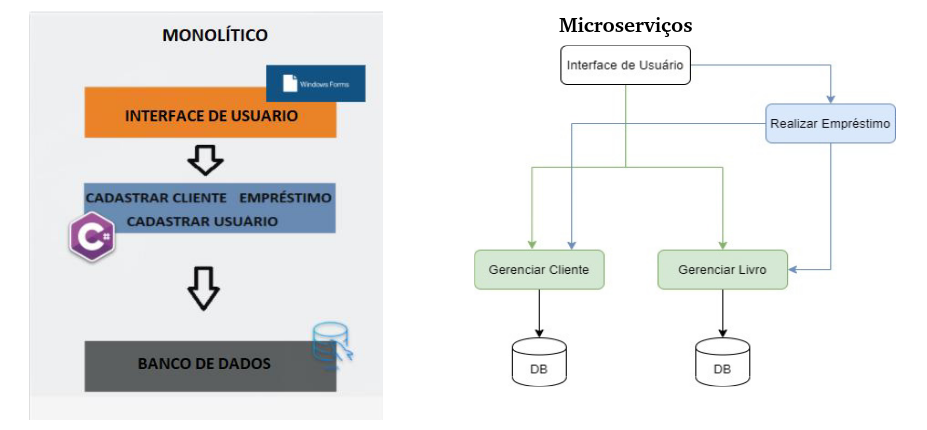
\includegraphics[width=1\textwidth]{./img/monolito-e-microservicos.png}
		\caption{Monolítico e Microsserviços
			Adaptado de \cite{garcia2021}}
		\label{fig:exampleFig1}
	\end{figure}
	
	%ACHO QUE AQUI BUSCAR ALGUMA IMAGEM COMPARANDO MONOLITOS E MICROSERVICOS
	
	Empresas como Netflix e Walmart adotaram a arquitetura de microsserviços para lidar com altos volumes de tráfego e demandas de escalabilidade, resultando em economias de recursos e melhor desempenho operacional. A Walmart, por exemplo, economizou muito o poder de computação após a migração, enquanto a Netflix usa mais de 500 microsserviços para lidar com bilhões de solicitações diárias \cite{castro2021}.
	
	\subsection{Desafios da Implementação de Microsserviços}
	
	Embora os microsserviços ofereçam muitos benefícios, sua implementação não está isenta de desafios. A complexidade de gerenciar múltiplos serviços independentes pode aumentar a dificuldade na resolução de problemas, como destacado em estudos recentes, grande parte dos entrevistados relataram dificuldades na identificação de causas de erros em ambientes de microsserviços \cite{castro2021}. Assim, é essencial que as empresas se preparem adequadamente para essa transição, adotando práticas de monitoramento e integração contínua.
	
	
	\subsection{Características dos Microserviços}
	Entre as principais características dos microserviços estão:
	\begin{itemize}
		\item \textbf{Desacoplamento}: A independência entre serviços permite que os mesmos sejam desenvolvidos, atualizados e escalados de maneira isolada, promovendo maior flexibilidade no desenvolvimento.
		\item \textbf{Escalabilidade Independente}: Cada serviço pode ser escalado de acordo com suas necessidades específicas, otimizando o uso de recursos do sistema.
	\end{itemize}
	
	\section{Integração entre REST e Microsserviços}
	
	A combinação de REST com Microserviços permite uma abordagem modular e eficiente, ideal para ambientes de sistemas distribuídos. O uso de APIs RESTful como interface para comunicação entre microserviços é amplamente adotado devido à simplicidade e interoperabilidade oferecidas \cite{newman2015}.
	
	\subsection{Benefícios da Integração}
	A combinação de microserviços com REST facilita a escalabilidade, a manutenção e a evolução contínua dos sistemas, uma vez que cada microsserviço pode ser desenvolvido, implantado e escalado de forma independente, enquanto o REST garante a interoperabilidade e a simplicidade na comunicação entre eles. Isso se deve principalmente aos seguintes motivos:
	\paragraph{Interface Uniforme}: O uso de APIs REST entre microserviços proporciona uma interface clara e padronizada para a comunicação entre diferentes componentes do sistema.
	\paragraph{Escalabilidade e Desempenho}: Microserviços com comunicação baseada em REST podem ser escalados independentemente, enquanto o uso de cache e a arquitetura stateless garantem desempenho eficiente \cite{cavaleiro2013}.
	
	\section{Conclusão}
	
	Os Princípios REST, quando aplicados a uma Arquitetura de Microserviços, fornecem uma base robusta para sistemas distribuídos modernos. Embora tanto a Arquitetura REST quando os Microsserviços apresentem desafios, como a gestão de segurança e complexidade operacional, os benefícios em termos de escalabilidade, resiliência e flexibilidade superam as dificuldades, permitindo o desenvolvimento de sistemas adaptáveis e resilientes \cite{fielding2000}.
	
	
	\bibliographystyle{sbc}
	\begin{thebibliography}{99}
		\bibitem{cavaleiro2013} CAVALEIRO, A. F. S. *Estilo Arquitetural REST para Criação de Web Services*. Fundação Educacional do Município de Assis, 2013.
		\bibitem{fielding2000} FIELDING, R. T. *Architectural Styles and the Design of Network-based Software Architectures*. University of California, 2000.
		\bibitem{newman2015} NEWMAN, S. *Building Microservices: Designing Fine-Grained Systems*. O'Reilly Media, 2015.
		\bibitem{castro2021} CASTRO, T. F. de S.; VALE, F. G. de M.; SOUSA, F. H. F. de. Microsserviços. *Brazilian Journal of Development*, v. 7, n. 3, p. 21829-21833, mar. 2021.
		\bibitem{newcomer2002} NEWCOMER, E. *Understanding Web Services: XML, WSDL, SOAP, and UDDI*. Addison-Wesley Professional, 2002.
		
		\bibitem{garcia2021} GARCIA, G. B. *Do monolítico ao microserviço A transformação das equipes e sistemas*. nstituto Federal de Educação, Ciência e Tecnologia de São Paulo, 2021.
				
	\end{thebibliography}
	
\end{document}
